\documentclass[10pt,a4paper,landscape,twocolumn]{article}
\usepackage[utf8]{inputenc}
\usepackage[czech]{babel}
\usepackage[T1]{fontenc}
\usepackage{amsmath}
\usepackage{amsfonts}
\usepackage{amssymb}
\usepackage{graphicx}
\usepackage[left=1cm,right=1cm,top=0cm,bottom=1cm]{geometry}
\title{Závěrečná fyzikální paralympiáda starších, LMFT 2020}
\date{}

\begin{document}

\maketitle
\thispagestyle{empty}

\section{CERN (7 bodů)}
Protony obíhají okruh o délce 27 km a na správné trase jsou udržovány homogenním magnetickým polem. Jak velký musí být vektor magnetické indukce a kam musí mířit, abychom dosáhli srážek o energii 125 GeV? Srážejí se vždy dva protony obíhající v opačném směru.

\section{Atraktivní ovce (9 bodů)}
Stokilová ovce se dotkla ohradníku a nabila se, a protože měla na nohách holinky, nevybila se. Jaký náboj musí mít, aby mezi ní a metr vzdáleným bačou, nabitým sto Coulomby, bylo dosaženo průrazného napětí a zajiskřilo to? Dielektrická pevnost vzduchu je $3~\mathrm{MV}\cdot\mathrm{m}^{-1}$.

\section{Odporný odpor (10 bodů)}
Spočtěte odpor soustavy stejných rezistorů o odporech $R$ na obrázku.
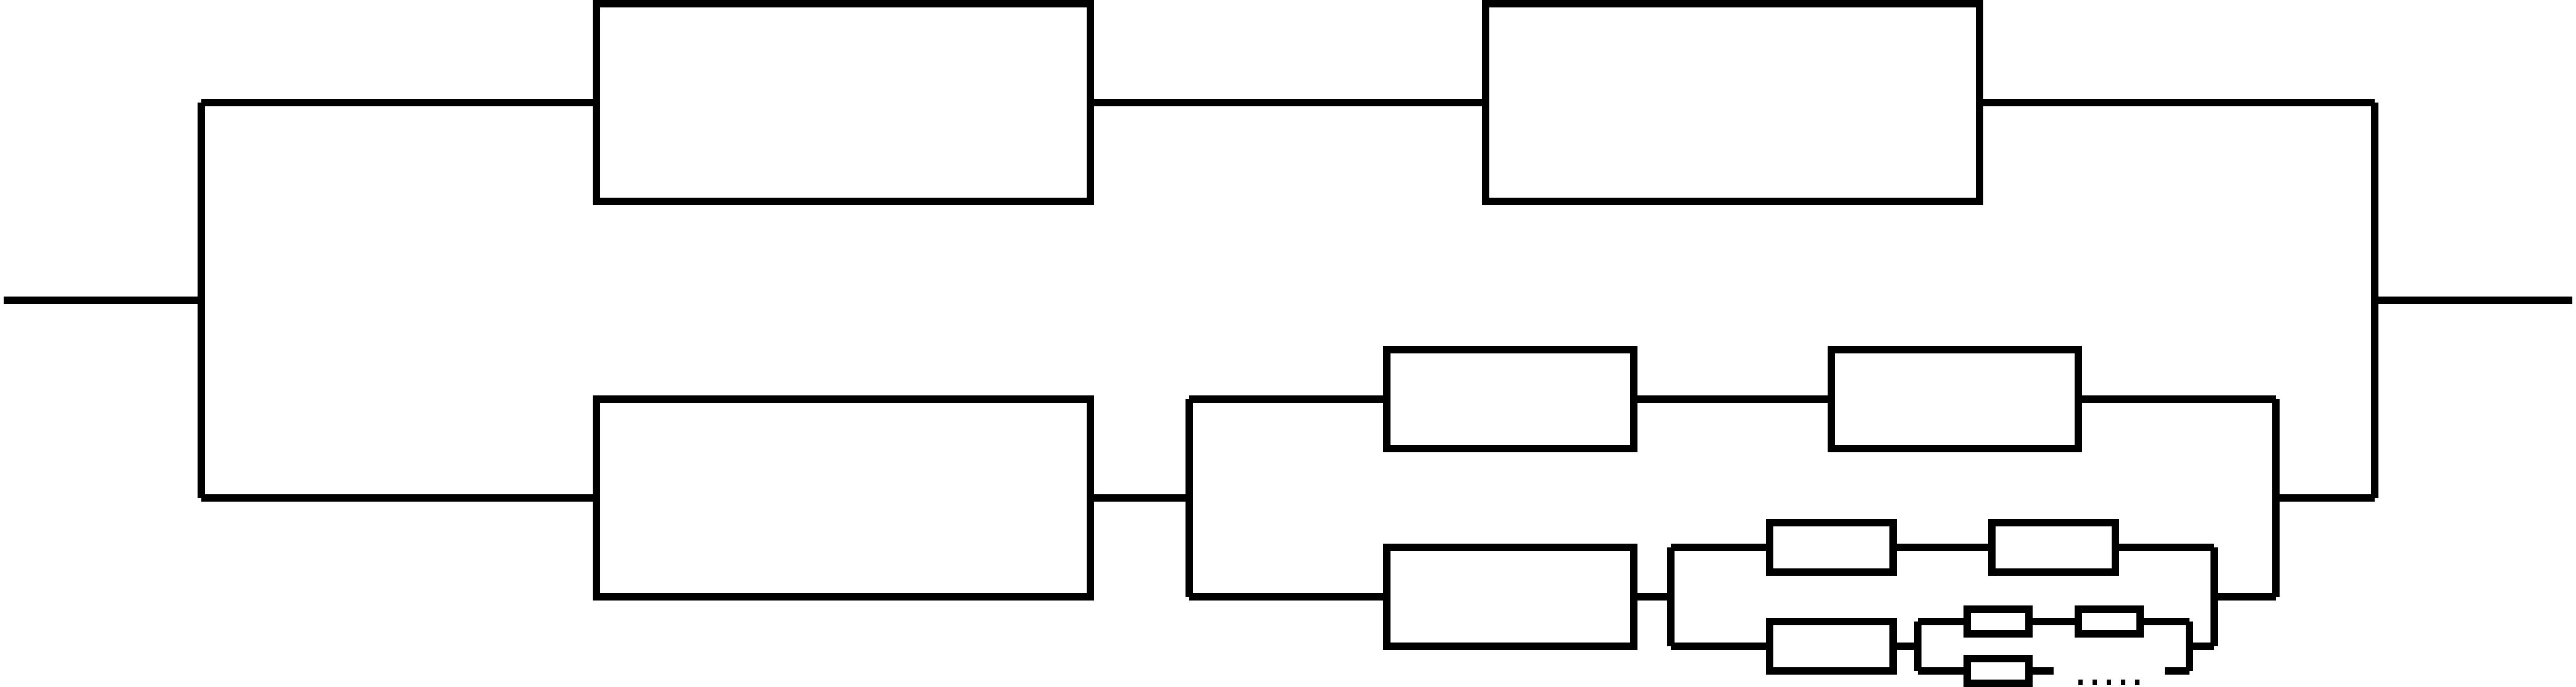
\includegraphics[scale=0.05]{img/odpor.jpg}

\section{Otáčení (9 bodů)}
Mějme vektorové pole v prostoru dané rovnicí
\begin{equation*}
\vec{E}\left(x, y, z\right) = \left(\frac{4xy}{z}, \frac{2x^2}{z}, -\frac{2x^2y}{z^2} - z^3\right)~.
\end{equation*}
Rozhodněte, zda má potenciál, a pokud má, určete jej. (Pokud nemá, nemusíte jej určovat.)

\section{Koule v neviskózní kapalině (12 bodů)}
Dvě stejné kuličky ve vzduchu jsou nabité stejným elektrickým nábojem a jsou zavěšeny ve stejném bodě na dvou stejně dlouhých nitích, které spolu svírají úhel $2\alpha$ (náboj je dostatečně velký, aby se kuličky nedotýkaly). Nyní je ponoříme do benzenu o hustotě $\rho_b = 879~\mathrm{kg}\cdot\mathrm{m}^{-3}$ a relativní permitivitě $\epsilon_r = 2.3$ a po ponoření se úhel mezi nimi nezmění. Jaká je hustota kuliček?

\section{Koule ve viskózní kapalině (14 bodů)}
V nádobě s ricinovým olejem o dynamické viskozitě $\eta$, která je ve stavu beztíže, urychlujeme kuličku o náboji $Q$ a poloměru $r$ homogenním a konstantním elektrickým polem $\vec{E}$, které míří ve směru osy $x$. Naopak ji brzdí Stokesův odpor $\vec{F} = -6\pi\eta r\vec{v}$, jedná se tedy o jednorozměrnou úlohu. Určete rychlost v ustáleném stavu (když se pohybuje rovnoměrně). Určete závislost polohy kuličky na čase, pokud se na počátku pohybuje ustálenou rychlostí a pole vypneme. Jak daleko se dostane? Vyhodnoťte pro $\eta = 987\cdot 10^{-3}~\mathrm{Pa}\cdot\mathrm{s}^{-1}$, $r = 5~\mathrm{mm}$, $E = 20~\mathrm{m}\cdot\mathrm{s}^{-1}$ a $Q = 0.1~\mathrm{C}$.

\section{Nabitý prostor (10 bodů)}
Spočtěte rozložení náboje v prostoru, víte-li, že potenciál klesá se vzdáleností $r$ od počátku souřadné soustavy jako
\begin{equation*}
\varphi = U_0 e^{-r/l}~,
\end{equation*}
kde $U_0$ a $l$ jsou konstanty.

\section{Na teplotě nezáleží (10 bodů)}
Na jednom konci válcového měděného vodiče o odporu 10 $\Omega$ (při teplotě $0^\circ\mathrm{C}$) je udržována teplota $20^\circ\mathrm{C}$, na druhém konci teplota $400^\circ\mathrm{C}$. Určete odpor vodiče, jestliže teplota podél něj klesá rovnoměrně.

\section{Tripólis (10 bodů)}
Spočtěte intenzitu lineárního trojpólu, kde náboj $2Q$ je v počátku souřadné soustavy a dva náboje $-Q$ jsou symetricky na ose $x$ v malé vzdálenosti od počátku. Přibližte do podobného tvaru jako u dipólu.

\section{Suchá úloha (9 bodů)}
Nekonečná rovinná deska o tloušťce $a$ je rovnoměrně nabita nábojem s objemovou hustotou $\rho$. Najděte intenzitu a potenciál elektrického pole ve vzdálenosti $z$ od středu desky jak uvnitř, tak vně.

\end{document}